\section{Facit}

\setcounter{opgave}{0}

\begin{opgave}{Det Galileiske Relativitetsprincip}
    \opg Siden toget kører med konstant hastighed, svarer det til at det er i hvile, her falder stenen med konstant acceleration;
    $$
        y'=y'_0-\frac{gt^2}{2}
    $$
    \opg Gallilei transformationen virker kun langs bevægelsen, så faldet er det samme set fra en observatør på jorden. Er toget $S'$ og jorden $S$, er den vandrette bevægelse efter Gallilei transformationen, hvis stenen starter i nul:
    $$
        x=vt
    $$
\end{opgave}

\begin{opgave}{Tog}
    En billetkontrolør går ned igennem et tog \SI{100}{m} langt tog.
    \opg Hvis kotroløren går med en hastighed på $u=\SI{1}{\frac{m}{s}}$, hvor langt tid tager det kontroløren at gå fra bagenden til forenden af toget?
    
    Kontrolørens bevægelse i toget er
    $$
        x'=ut'
    $$
    Sættes $x'=L$ og isoleres tiden findes
    $$
        t'=\frac{L}{u}=\SI{100}{s}
    $$
    
    Toget kører med en hastighed på $v=\SI{20}{\frac{m}{s}}$ (\SI{72}{\frac{km}{h}}).
    \opg  Brug Galilei transformationen til at finde ud af hvor lang kontroløren har bevæget sig i forhold til omgivelserne.
    
    Vi kender koordinaterne i $S'$:
    \begin{align*}
        x'&=L\\
        t'&=\frac{L}{u}
    \end{align*}
    Galilei transformationen fra $S'$ til $S$ er
    \begin{align*}
        x&=x'+vt'\\
        t&=t'
    \end{align*}
    Så kontroløren har rejst
    $$
        x=x'+vt'=L+\frac{v}{u}L=\left(1+\frac{v}{u}\right)L=\SI{2100}{m}
    $$
\end{opgave}

\begin{opgave}{Kombination af Galileitransformationer}
    Til at starte med er Gallilei transformationen fra $S$ til $S'$
    \begin{align*}
        x'=x-vt\\
        t'=t
    \end{align*}
    Tiden er absolut efter Gallilei transformationen, så
    $$
        t=t'=t''
    $$
    \opg Gallileitransformationen fra $S$ til $S''$ er på samme form, bare med $u$ i stedet for $v$
    $$
        x''=x-ut
    $$
    \opg Vi kan beskrive $x$ ud fra $x''$, 
    $$
        x=x''+ut
    $$
    Dette kan sættes ind i Gallilei transformationen imellem $S$ og $s''$
    $$
        x'=x''+ut-vt
    $$
    Hvilket kan omarrangeres til 
    $$
        x''=x'-(u-v)t
    $$
    \opg $u-v$ er hastigheden af $S''$ i forhold til $S$.
\end{opgave}

\begin{opgave}{Myoner i atmosfæren}
    \opg Her bruges tidsforlængelsesformlen (5.7)
    $$
        T=T_0\gamma=\frac{T_0}{\sqrt{1-\frac{v^2}{c^2}}}=\frac{\SI{1,5}{\mu s}}{\sqrt{1-\frac{0,99^2c^2}{c^2}}}=\SI{10,6}{\mu s}
    $$
    \opg For at finde halveringslængden multipliceres hastigheden med halveringstiden.
    $$
    \ell_{1/2}=T_{1/2}\cdot 0.99 c=\SI{3158}{m}
    $$
    \opg Antallet af halveringslængder ned til jordoverfladen er
    $$
    \frac{\SI{10}{km}}{\ell_{1/2}}=3,158
    $$
    Så for at finde hvor stor en andel af myonerne der når jordoverfladen opløftes en halv i dette antal
    $$
    f=\left(\frac{1}{2}\right)^{3,158}=11,1\%
    $$
\end{opgave}

\begin{opgave}{Pioner i atmosfæren}
    De tre første delopgaver er identiske med den forrige opgave, med en anden halveringstid.
    \opg 
    $$
    T_{1/2}=\gamma T'=\SI{127,6}{\mu \second}
    $$
    \opg
    $$
    \ell_{1/2}=T_{1/2}\cdot 0.99 c=\SI{3,70}{m}
    $$
    \opg
    $$
    \frac{\SI{10}{km}}{\ell_{1/2}}=2639
    $$
    $$
    \left(\frac{1}{2}\right)^{2639}=3,8\cdot 10^{-795}
    $$
    En del regnemaskiner vil her bare sige nul.
    \opg
    Effektivt set vil ingen pioner nå overfladen.
\end{opgave}

\begin{opgave}{Relativistisk Usain Bolt}
\begin{align*}
    L&=\SI{100}{m}
    v&=\SI{12,4}{\frac{m}{s}}
    T&=\SI{9,572}{s}
    c&=\SI{3e8}{\frac{m}{s}}
\end{align*}
    \opg
    $$
    L'=\frac{L}{\gamma}=L\sqrt{1-\frac{v^2}{c^2}}=\SI{99.999999999999914578}{m}
    $$
    \opg
    $$
    T'=T\gamma=\frac{T}{1-\frac{v^2}{c^2}}=\SI{9.572}{s}
    $$
    \opg 
    $$
    c=\SI{15}{\frac{m}{s}}
    $$
    $$
    L'=\frac{L}{\gamma}=\SI{56,27}{m}
    $$
    $$
    T'=T\gamma=\SI{17}{s}
    $$
\end{opgave}

\begin{opgave}{Myonens rejse}
    \opg
    De \SI{10}{km} længdeforkortes
    $$
    L'=\frac{L}{\gamma}=L\sqrt{1-\frac{v^2}{c^2}}=\SI{1,41}{km}
    $$
    \opg
    Med en hastighed på $0,99 c$ tager det myonen
    $$
    \frac{L'}{v}=\SI{4,8}{\mu s}
    $$
    Andelen der når ned er
    $$
    \left(\frac{1}{2}\right)^{\SI{4,8}{\mu s}/\SI{1,5}{\mu s}}=11\%
    $$
    Med flere decimaler kan det godt være at dette ikke er helt det samme som i opgave 5,4, det skyldes afrunding.
\end{opgave}

\begin{opgave}{Lorentztranformation af forskelle}
    \opg Det er blot forskellen i mærkekordinaterne
    \begin{align*}
        \Delta x'&=x'_2-x'_1\\
        \Delta t' &= x'_2-t'_1
    \end{align*}
    \opg $x'_1$, $x'_2$, $t_1'$ og $t_2'$ findes ud fra Lorentztransformation.
    \begin{align*}
        x'_1&=\gamma(x_1-vt_1)\\
        t'_1&=\gamma\left(t_1-\frac{x_1t}{c^2}\right)\\
        x'_2&=\gamma(x_2-vt_2)\\
        t'_2&=\gamma\left(t_2-\frac{x_2t}{c^2}\right)
    \end{align*}
    
    Så er $\Delta x'$
    $$
    \Delta x'=x_2'-x_1'=\gamma (x_2-vt_2-x_1+vt_2)=\gamma(\Delta x-v\Delta t)
    $$
    og $\Delta t'$ 
    $$
    \Delta t'=\gamma\left(t_2-\frac{vx_1}{c^2}-t_1+\frac{vx_2}{c^2}\right)=\gamma\left(\Delta t-\frac{\Delta xv}{c^2}\right)
    $$
    Transformationen af forskellene er identisk med transformationen af koordinaterne.
\end{opgave}

\begin{opgave}{Tidsforlængelse og længdeforkortelse i Lorentztransformationerne}
    Her bruger vi Lorentztransformationen for forskelle
    \begin{align*}
        \Delta x'&=\gamma(\Delta x-v\Delta t)\\
        \Delta t'&=\gamma \left(\Delta t-\frac{\Delta xv}{c^2}\right)
    \end{align*}
    \opg Sættes $\Delta t$ til nul bliver $x$ ligningen til ligningen ligningen for længdeforkortelse.
    $$
    \frac{\Delta x'}{\gamma}=\Delta x
    $$
    Hvor $\Delta x'$ er $L_0$ og $\Delta x$ er $L$.
    \opg 
    Sættes $\Delta x$ til nul vil $t$-ligningen blive
    $$
    \Delta t'=\gamma \Delta t
    $$
    hvor $\Delta t'=T$ og $\Delta t=T_0$.
    \opg
    For at $\Delta x$ skal være nul skal
    $$
    x_1=x_2
    $$
    Tilsvarende for $\Delta t$ skal
    $$t_1=t_2$$
\end{opgave}

\begin{opgave}{Tjek af Lorentztransformationerne}
    \opg 
     $\gamma$-faktoren differentieres efter kædereglen
     $$
     \dv{\gamma}{v}=\frac{-2v}{2c^2}\left(1-\frac{v^2}{c^2}\right)^{-3/2}=\frac{-v}{c^2}\left(1-\frac{v^2}{c^2}\right)^{-3/2}
     $$
     \opg
     For $v=0$ bliver 
     $$\gamma(0)=1$$
     og
     $$
     \dv{\gamma}{v}=0
     $$
     Så for små hastigheder er $\gamma$-faktoren
     $$
     \gamma\approx 1
     $$
     \opg 
     Det giver Lorentztransformationen
     \begin{align*}
         x'=\gamma(x-vt)\approx -vt\\
         t'=\gamma\left(t-\frac{vx}{c^2}\right)\approx t
     \end{align*}
     Andet led i $t$ ligningen forsvinder fordi $v$ er meget mindre end $c$.
     
     Dette efterlader Gallileitransformationen.
     \opg
     Den andenafledte af gammafaktoren er, efter kædereglen og produktreglen,
     $$
     \dv[2]{\gamma}{v}=\frac{1}{c^2}\left(1-\frac{v^2}{c^2}\right)^{-3/2}-\frac{3v^2}{c^4}\left(1-\frac{v^2}{c^2}\right)^{-5/2}
     $$
     Tilnærmelsen af $\gamma$-faktoren er så
     $$
     \gamma\approx 1+\frac{v^2}{2c^2}
     $$
     Så er andenordens tilnærmelsen af Lorentztransformationen
     \begin{align*}
         x'&\approx x-vt+\frac{xv^2}{2c^2}-\frac{v^3t}{c^2}\approx x-vt-\frac{v^3t}{c^2}\\
         t'&\approx t-\frac{xv}{c^2}+\frac{tv^2}{2c^2}-\frac{xv^3}{c^2}\approx t-\frac{xv}{c^2}-\frac{xv^3}{c^2}
     \end{align*}
\end{opgave}


\begin{opgave}{Addition af hastigheder}
    \opg Personens bevægelse i $S'$ er
    $$
    x'=ut'.
    $$
    \opg
    Galilei transformationen fra $S'$ til $S$ er
    \begin{align*}
        x&=x'+vt\\
        t&=t'
    \end{align*}
    Hvilket betyder at personens bevægelse i $S$ er
    \begin{align*}
        x&=ut'+vt'\\
        t&=t'
    \end{align*}
    Så personens bevægelse er
    \[
    x=(u+v)t
    \]
    \opg
    Lorentztransformationen fra $S'$ til $S$ er
    \begin{align*}
        x&=\gamma(x'+vt')\\
        t&=\gamma\left(t'+\frac{x'v}{c^2}\right)
    \end{align*}
    Indsættes personens bevægelse i $S'$ bliver det.
    \begin{align*}
        x&=\gamma (ut'+vt')=\gamma(u+v)t'\\
        t&=,\gamma\left(t'+\frac{uvt'}{c^2}\right)
    \end{align*}
    $t'$ kan isoleres i $t$-ligningen,
    \[
    t'=\dfrac{t}{\gamma\left(1+\dfrac{uv}{c^2}\right)}.
    \]
    Kombineres de to ligninger findes
    \[
    x=\dfrac{\gamma(u+v)t}{\gamma\left(1+\dfrac{vu}{c^2}\right)}=\dfrac{u+v}{1+\dfrac{uv}{c^2}}t
    \]
    Så set fra $S$ bevæger personen sig også med en konstant hastighed, og denne hastighed er
    \begin{equation}
    \dfrac{u+v}{1+\dfrac{uv}{c^2}}.\label{rel:hastadd}
    \end{equation}
    Denne ligning kaldes den relativistiske  hastighedsformel.
    Beværk at så længe både $u$ og $v$ er mindre end $c$ vil \eqref{rel:hastadd} også være det
    (sæt $c$ ind og tjek hvis du vil være sikker).
    \opg Når både $u$ og $v$ er meget mindre end $c$ vil $\frac{vu}{c^2}$ være meget lille, og \eqref{rel:hastadd} bliver
    \begin{equation*}
    \dfrac{u+v}{1+\dfrac{uv}{c^2}}\approx u+v.
    \end{equation*}
    Som vi ville forvente genfinder vi det klassiske udtryk for lave hastigheder.
\end{opgave}

\begin{opgave}{Jesus og Julius}
    Cæsar blev myrdet i 44 f.Kr., og afstanden imellem Rom og Bethlehem er ca. \SI{2300}{km}.
    \opg Findes der en iagttager, for hvilken Jesus' fødsel og Cæsars død var samtidige?
    
    Nej. Se begrundelse i det nedenstående spørgsmål.
    %
    \opg Hvorfor/hvorfor ikke?
    
    For at to begivenheder er samtidige vil $\Delta t = 0$. Rumtidsintervallet bliver derved
    \begin{align}
        \Delta s^2 &= \Delta x^2 - c^2 \Delta t^2 = \Delta x^2 \geq 0 \: ,
    \end{align}
    så hvis rumtidsintervallet bliver positivt, da vil der findes en observatør, der mener, at Jesus' fødsel og Cæsars død er sket samtidigt.
    
    Jesus blev født i år 0, mens Cæsar døde i år 44. Herved bliver $\Delta t = 44 \: \text{år}$. Afstanden mellem Rom og Bethlehem er $\Delta x = \SI{2300}{km}$. Rumtidsintervallet bliver derved
    \begin{align}
        \Delta s^2 &= (\SI{2300}{km})^2 - c^2 (44 \, \text{år})^2
            = (\SI{2300}{km})^2 - (44 \: \text{\lightyear})^2 \cdot \left(9.46 \cdot 10^12 \, \si{\kilo\metre\per\lightyear}\right)^2 \nonumber\\
            &= (\SI{2300}{km})^2 - (416,24 \cdot 10^12 \, \si{\kilo\metre})^2
            = (\SI{2300}{km})^2 - (4162,4 \cdot 10^11 \, \si{\kilo\metre})^2
            \leq 0 \: ,
    \end{align}
    hvor omregningen fra lysår til kilometer er $\SI{1}{\lightyear} = 9.46 \cdot 10^12 \, \si{\kilo\metre}$. Det kan ses at $\num{2300} < \num{4162,4}$, hvorved vi får et negativt rumtidsinterval -- også den store tierpotens giver dette ret meget.
    
    Det er altså ikke muligt for en observatør at se Jesus' fødsel og Cæsars død som samtidige.
\end{opgave}

\begin{opgave}{Fulbert sover længe}%til rumtidsintervallet
    Fulbert bor \SI{5}{km} fra skolen og har sat sit vækkeur, så han er klar til at tage af sted klokken kvart i otte, når han skal møde klokken otte.
    \opg Hvad er rumtidsintervallet $\Delta s^2$ imellem Fulbert er klar, og han skal møde?
    
    Det er givet, at $\Delta x = \SI{5}{\kilo\metre}$ og $\Delta t = \SI{15}{min}$:
    \begin{align}
        \Delta s^2 &= \Delta x^2 - c^2 \Delta t^2
            = (\SI{5}{\kilo\metre})^2 - c^2 (\SI{15}{min})^2 \nonumber\\
            &= \left(5 \cdot 10^3 \, \si{\metre}\right)^2 - \left(\SI{2,99792458}{\metre\per\second}\right)^2 \left(15 \cdot 60 \, \si{\second}\right)^2 \nonumber\\
            &= 5 \cdot 10^6 \, \si{\metre\squared} - \SI{269813212200}{\metre\squared}
            = \SI{-269808212200}{\metre\squared} \: .
    \end{align}
    \newline
    %
    Fulbert kan godt lide at sove længe, så de fleste dage tager han lidt ekstra tid under dynen, så han først er klar klokken otte.
    \opg Hvad er rumtidsintervallet så?
    
    Nu ændres tidsintervallet, så $\Delta t = 0$. Derved bliver rumtidsintervallet
    \begin{align}
        \Delta s^2 &= \Delta x^2 - c^2 \Delta t^2
            = \Delta x^2
            = (\SI{5}{\kilo\metre})^2
            = \left(5 \cdot 10^3 \, \si{\metre}\right)^2
            = 5 \cdot 10^6 \, \si{\metre\squared} \: .
    \end{align}
    \newline
    %
    Fulberts lærere er blevet trætte af, at han altid kommer for sent.
    De har sagt at han ikke må sove så længe, at det ikke er fysisk muligt for ham at være i skole til tiden.
    Som den aspirerende fysiker han er, tolker Fulbert det som at han ikke må overskride lysets hastighed.
    \opg Hvornår skal Fulbert senest være klar til at tage af sted, og hvor stort er rumtidsintervallet imellem at han tager af sted, og han skal være fremme?
    
    Fulbert bevæger sig altså med lysets hastighed, hvorved rumtidsintervallet må være $Delta s^2 = 0$. Dermed må
    \begin{align}
        \Delta x^2 &= c^2 \Delta t^2 \\
        \Rightarrow \Delta t &= \frac{\Delta x}{c} = \dfrac{\SI{5000}{\metre}}{\SI{299792458}{\metre\per\second}}
            = 16,7 \cdot 10^{-6} \, \si{\second}
            = \SI{16,7}{\micro\second} \: .
    \end{align}
    Fulbert skal altså gå hjemmefra (med lysets hastighed) \SI{16,7}{\micro\second} i 8 om morgenen.
\end{opgave}
    
\begin{opgave}{Fulbert på rumrejse} \label{opg:FulbertPaaRumrejse}
    Fulbert drager ud på en rumrejse imens Beatrice bliver tilbage på Jorden.
    Fulbert rejser med $0,8 c$, og rejser til Alfa Centauri, \SI{4,4}{\lightyear} borte.
    \opg Hvor lang er rejsen set fra Fulbert, når han er i bevægelse? 
    
    Til at beregne, hvor lang rejsen er for Fulbert (system $S'$), som er i bevægelse i forhold til Beatrice (system $S$), benyttes længdeforkortelse, ligning \ref{rel:Laengdeforkortelse}
    \begin{align}
        x' &= \frac{x}{\gamma}
            = \sqrt{1 - \frac{v^2}{c^2}} \cdot x
            = \sqrt{1 - \dfrac{(0,8c)^2}{c^2}} \cdot \SI{4,4}{\lightyear}
            = \sqrt{1 - (0,8)^2} \cdot \SI{4,4}{\lightyear} \nonumber\\
            &= \sqrt{1 - 0,64} \cdot \SI{4,4}{\lightyear}
            = \sqrt{0,36} \cdot \SI{4,4}{\lightyear}
            = 0,6 \cdot \SI{4,4}{\lightyear}
            = \SI{2,64}{\lightyear} \: .
    \end{align}
    %
    \opg Hvor lang tid tager Fulberts rejse for ham?
    
    Tiden, som Fulbert ser, at rejsen vil tage for ham, må være givet, som i klassisk mekanik, som sted delt med hastighed
    \begin{align}
        t'= \frac{x'}{v} = \frac{\SI{2,64}{ly}}{0,8c} = \frac{2,64 \, \text{år}}{0,8} = 3,3 \, \text{år} \: .
    \end{align}
    %
    \opg Hvor lang tid tager rejsen set fra Beatrice?
    
    Til at beregne tiden, som rejsen tager, set fra Beatrice, kan man gøre en af to ting:
    \begin{enumerate}
        \item Enten kan man gøre som i opgave \thechapter,\ref{opg:FulbertPaaRumrejse} delopgave 2, bare ved brug af afstanden, som Beatrice observerer:
        \begin{align}
            t = \frac{x}{v} = \frac{\SI{4,4}{\lightyear}}{0,8c} = \frac{4,4 \, \text{år}}{0,8} = 5,5 \, \text{år}
        \end{align}
        \item Eller man kan benytte sig af tidsforlængelse, ligning \ref{rel:Tidsforlaengelse}, og den tid, som Fulbert observerer, at rejsen tager. Her kender vi tiden, som Fulbert mener, at rejsen vil tage, hvilket i ligning \ref{rel:Tidsforlaengelse} vil være $T_0$, da vi har regnet det i Fulberts hvilesystem, så vil tiden, som Beatrice mener, at turen tager -- i ligning \ref{rel:Tidsforlaengelse} $T$ -- være
        \begin{align}
            t &= \gamma t'
                = \dfrac{1}{\sqrt{1 - \dfrac{v^2}{c^2}}} t'
                = \dfrac{3,3 \, \text{år}}{\sqrt{1 - \frac{(0,8)^2}{c^2}}}
                = \frac{3,3 \, \text{år}}{\sqrt{1 - 0,64}}
                = \frac{3,3 \, \text{år}}{\sqrt{0,36}}
                = \frac{3,3 \, \text{år}}{0,6}
                = 5,5 \, \text{år} \: .
        \end{align}
    \end{enumerate}
    %
    \opg Fulbert vender hjemad lige efter han er nået frem. Hvor lang tid har hele rejsen taget for Fulbert?
    
    Idet Fulbert vender om med det samme, at han når stjernen, så vil tiden blot være den dobbelte af tiden fundet i opgave \thechapter,\ref{opg:FulbertPaaRumrejse} delopgave 2, da dette blot var tiden den ene vej:
    \begin{align}
        t'_{tot} &= 2 t'
            = 2 \cdot 3,3 \, \text{år}
            = 6,6 \, \text{år} \: .
    \end{align}
    %
    \opg Hvor lang tid har Beatrice måttet vente på Jorden?
    
    Som i opgave \thechapter,\ref{opg:FulbertPaaRumrejse} delopgave 4 vil hele rejsen, set fra Beatrice, have taget det dobbelte af tiden, som rejsen tog den ene vej (fra \thechapter,\ref{opg:FulbertPaaRumrejse} delopgave 3):
    \begin{align}
        t_{tot} &= 2 t
            = 2 \cdot 5,5 \, \text{år}
            = 11 \text{år} \: .
    \end{align}\\
    
    Den opmærksomme læser vil opdage, at Fulbert og Beatrice oplever, at Fulberts rejse har varet to forskellige tider, hhv. $6,6$ år og $11$ år set fra hhv. Fulbert og Beatrice. Dette kaldes \emph{tvillingeparadokset}, da vi jo ikke kan have, at vi får forskellige resultater baseret på, hvilket referencesystem vi regner i. Selvom dette kaldes et paradoks, så er dette nu ikke tilfældet. Grunden til, at det ligner et paradoks er, at man antager, at Fulbert øjeblikkeligt kan vende om, når han når til stjernen. Vi har ikke taget højde for, at når man vender fra at rejse den éne vej til den anden, så decelererer og accelererer Fulberts rumskib. Dette har vi imidlertid ikke taget højde for, da acceleration ikke kan beskrives i den specielle relativitetsteori men kun i den generelle relativitetsteori. Medregnes denne acceleration viser det sig, at Fulbert og Beatrice er enige om, hvor lang tid, som Fulberts rejse har taget, hvorved ''paradoks''-delen forsvinder.
\end{opgave}


\begin{figure}[t]
    \centering
    \begin{subfigure}[t]{.45\textwidth}
        \centering
        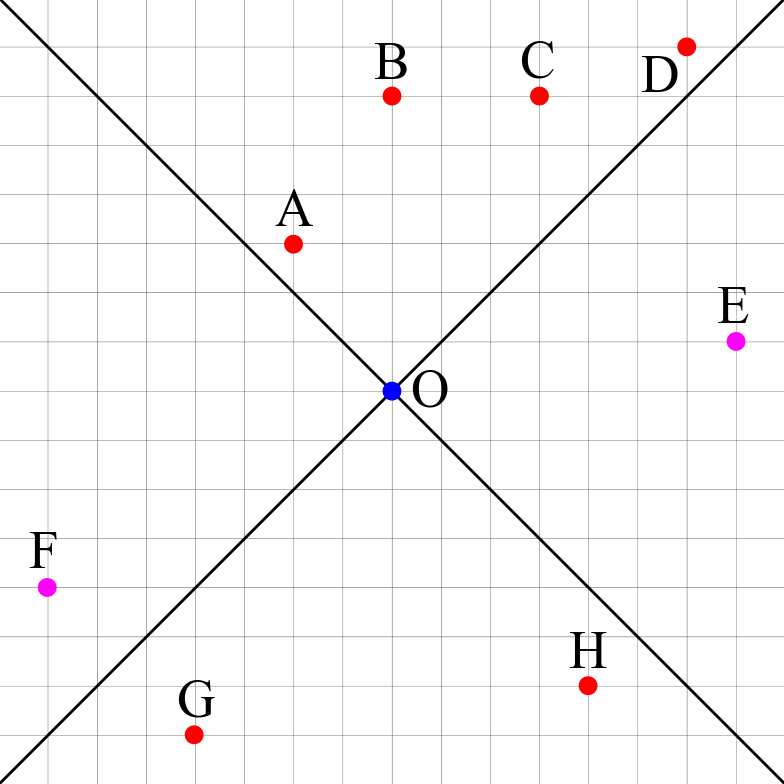
\includegraphics[width=\columnwidth]{facit/figurer/SR/LyskegleFacit1.png}
        \caption{Facit for opgave \ref{opg:LyskeglenFacit} delopgave 1 og 2. De røde punkter er tidadskilte begivenheder ift. begivenhed $O$, og de lilla punkter er rumadskilte begivenheder ift. begivenhed $O$.}
        \label{fig:LyskeglenFacit1}
    \end{subfigure}
    \hfill
    \begin{subfigure}[t]{.45\textwidth}
        \centering
        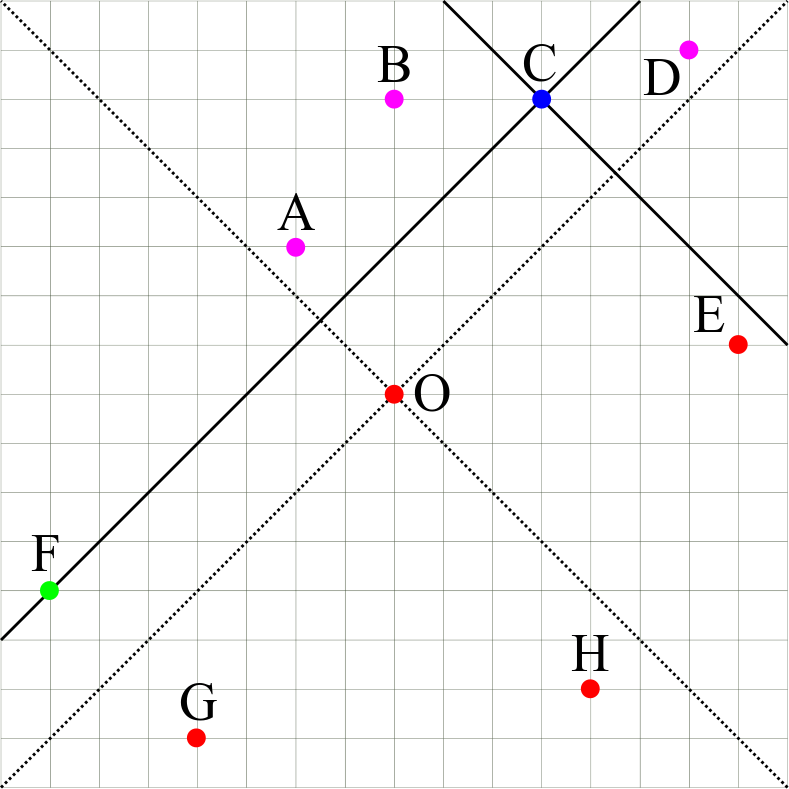
\includegraphics[width=\columnwidth]{facit/figurer/SR/LyskegleFacit3.png}
        \caption{Facit for opgave \ref{opg:LyskeglenFacit} delopgave 1 og 2. De røde punkter er tidadskilte begivenheder ift. begivenhed $O$, og de lilla punkter er rumadskilte begivenheder ift. begivenhed $O$. Det grønne punkt $F$ er \emph{lysadskilt}, hvorfor dette hverken kan ombyttes rummeligt eller tidsligt.}
        \label{fig:LyskeglenFacit2}
    \end{subfigure}
    \caption{Facit for opgave \thechapter,\ref{opg:LyskeglenFacit}.}
    \label{fig:LyskeglenFacit}
\end{figure}

\begin{opgave}{Lyskeglen} \label{opg:LyskeglenFacit}
Vi betragter begivenhederne indtegnet på figur \ref{fig:LyskegleOpgave}, som viser lyskeglen for med begivenheden $O$ som nu og her.
\opg Hvilke begivenheder kan ske på samme sted som begivenhed $O$, hvis observatøren er i bevægelse?

For at to begivenheder kan ske på samme sted for en observatør i bevægelse, så skal begivenhederne være tidadskilte. For begivenhed $O$ vil de tidadskilte begivenheder ligge i for- eller fremtiden, hvorfor der er tale om begivenhederne $A$, $B$, $C$, $D$, $G$ og $H$. Dette er indtegnet på figur \ref{fig:LyskeglenFacit1} som de røde punkter.
%
\opg Hvilke begivenheder kan ske på samme tidspunkt som begivenhed $O$, hvis observatøren er i bevægelse?

For at to begivenheder kan ske til samme tid for en observatør i bevægelse, så skal begivenhederne være rumadskilte. For begivenhed $O$ vil de rumadskilte begivenheder ligge udenfor lyskeglen, hvorfor der er tale om begivenhederne $E$, og $F$. Dette er indtegnet på figur \ref{fig:LyskeglenFacit1} som de lilla punkter.
%
\opg Tegn en lyskegle for begivenhed $C$.

Lyskeglen for begivenhed $C$ er indtegnet på figur \ref{fig:LyskeglenFacit2} som de fuldtoptrukne linjer.
%
\opg Gentag delopgave 1 og 2 for begivenheden $C$.

Begivenhederne som kan foregå på samme sted som $C$ for en observatør i bevægelse, altså begivenheder, som ligger indenfor lyskeglen med $C$ som her og nu, er $E$, $O$, $G$ og $H$. Begivenhederne som kan foregå til samme tid som $C$ for en observatør i bevægelse, altså begivenheder, som ligger udenfor lyskeglen med $C$ som her og nu, er $A$, $B$, $D$ og $H$. Punktet $F$ er \emph{lysadskilt}, hvorfor dette hverken kan rummeligt eller tidsligt ombyttes.
\end{opgave}